\documentclass[border=4pt]{standalone}
% Shared TikZ macros for the "Gaussian wave" amplitude diagrams.
% Each wave is drawn isolated inside a fixed-size cell, no axes, with an
% optional probability label placed just outside the bump.
\usepackage{tikz}
\usepackage{amssymb}
\usepackage{amsmath}
\usetikzlibrary{calc,arrows.meta}

\definecolor{waveblue}{HTML}{3A7CA5}
\definecolor{wavered}{HTML}{D1495B}

% \gaussiancell{x0}{y0}{sign}{height}{color}{basislabel}{highlight}{problabel}
% Draws one Gaussian bump centered at (x0,y0), cell width 2.4, height range +-1.1.
% sign: +1 upright, -1 flipped. height: 0..1 (fraction of max bump height 0.85).
% basislabel: basis-state ket, always placed BELOW the baseline; empty string = no label.
% highlight: 1 draws a thin colored box around the cell, 0 = none.
% problabel: probability value, always placed ABOVE the bump's peak; empty string = no label.
\newcommand{\gaussiancell}[8]{%
  \begin{scope}[shift={(#1,#2)}]
    \pgfmathsetmacro{\amp}{#4*0.85*#3}
    \pgfmathsetmacro{\wid}{0.30}
    \draw[black, line width=0.5pt] (-1.15,0) -- (1.15,0);
    \draw[#5, line width=1.3pt, samples=120, smooth, domain=-1.05:1.05]
      plot (\x, {\amp*exp(-(\x*\x)/(2*\wid*\wid))});
    \fill[#5, opacity=0.18, samples=120, domain=-1.05:1.05]
      plot (\x, {\amp*exp(-(\x*\x)/(2*\wid*\wid))}) -- (1.05,0) -- (-1.05,0) -- cycle;
    \ifnum#7=1
      \draw[wavered, line width=0.9pt] (-1.15,-0.65) rectangle (1.15,1.35);
    \fi
    \ifx&#6&
    \else
      \ifnum#3>0
        \node[anchor=north, font=\footnotesize] at (0, -0.35) {#6};
      \else
        \node[anchor=north, font=\footnotesize] at (0, -0.95) {#6};
      \fi
    \fi
    \ifx&#8&
    \else
      \node[anchor=south, font=\small] at (0, 0.95) {#8};
    \fi
  \end{scope}
}

% \wavegrid{rows}{cols}{dx}{dy}{cellfn} where cellfn takes (row,col,index)
% (grid layout handled inline per-figure instead, for full control over per-cell content)

% \meanline{x0}{y0}{width}{amp}{label}
% Draws a dotted horizontal line at height amp (in the same units as
% \gaussiancell's amplitude, i.e. peak height = 0.85 at amp=1) spanning
% `width` cells wide, centered at (x0,y0), with a small label to its right.
\newcommand{\meanline}[5]{%
  \begin{scope}[shift={(#1,#2)}]
    \pgfmathsetmacro{\amp}{#4*0.85}
    \draw[gray, line width=0.9pt, densely dotted] (-1.15,\amp) -- (#3-1.15,\amp);
    \ifx&#5&
    \else
      \node[gray, anchor=west, font=\footnotesize] at (#3-1.05,\amp) {#5};
    \fi
  \end{scope}
}

\begin{document}
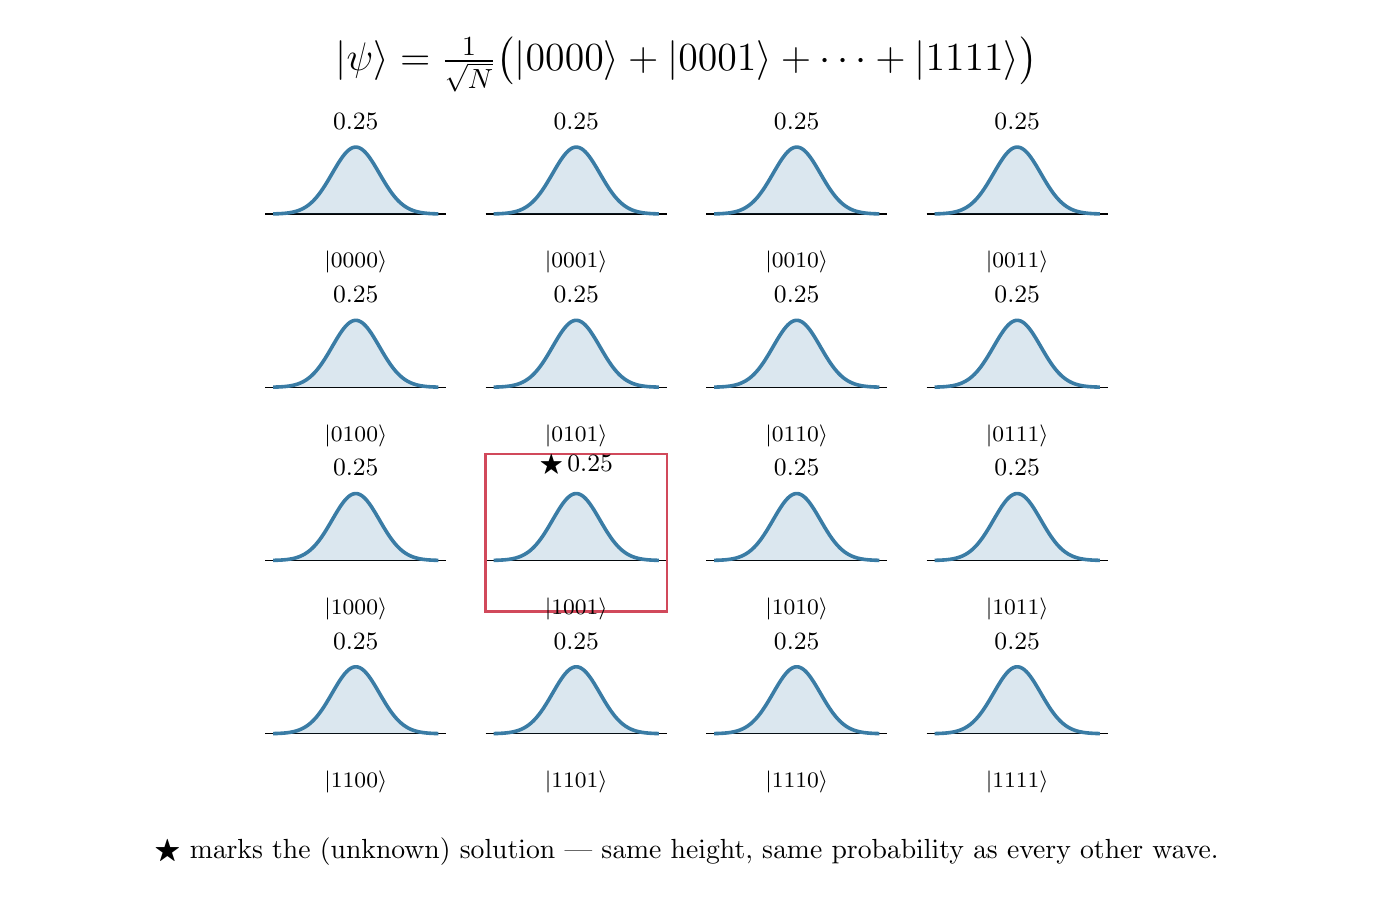
\begin{tikzpicture}
  \node[font=\Large] at (4.2, 9.9) {$|\psi\rangle = \tfrac{1}{\sqrt{N}}\big(|0000\rangle + |0001\rangle + \cdots + |1111\rangle\big)$};

  % Row 1
  \gaussiancell{0}{8.0}{1}{1}{waveblue}{$|0000\rangle$}{0}{$0.25$}
  \gaussiancell{2.8}{8.0}{1}{1}{waveblue}{$|0001\rangle$}{0}{$0.25$}
  \gaussiancell{5.6}{8.0}{1}{1}{waveblue}{$|0010\rangle$}{0}{$0.25$}
  \gaussiancell{8.4}{8.0}{1}{1}{waveblue}{$|0011\rangle$}{0}{$0.25$}

  % Row 2
  \gaussiancell{0}{5.8}{1}{1}{waveblue}{$|0100\rangle$}{0}{$0.25$}
  \gaussiancell{2.8}{5.8}{1}{1}{waveblue}{$|0101\rangle$}{0}{$0.25$}
  \gaussiancell{5.6}{5.8}{1}{1}{waveblue}{$|0110\rangle$}{0}{$0.25$}
  \gaussiancell{8.4}{5.8}{1}{1}{waveblue}{$|0111\rangle$}{0}{$0.25$}

  % Row 3 -- second cell is the highlighted (unknown) solution
  \gaussiancell{0}{3.6}{1}{1}{waveblue}{$|1000\rangle$}{0}{$0.25$}
  \gaussiancell{2.8}{3.6}{1}{1}{waveblue}{$|1001\rangle$}{1}{$\bigstar\,0.25$}
  \gaussiancell{5.6}{3.6}{1}{1}{waveblue}{$|1010\rangle$}{0}{$0.25$}
  \gaussiancell{8.4}{3.6}{1}{1}{waveblue}{$|1011\rangle$}{0}{$0.25$}

  % Row 4
  \gaussiancell{0}{1.4}{1}{1}{waveblue}{$|1100\rangle$}{0}{$0.25$}
  \gaussiancell{2.8}{1.4}{1}{1}{waveblue}{$|1101\rangle$}{0}{$0.25$}
  \gaussiancell{5.6}{1.4}{1}{1}{waveblue}{$|1110\rangle$}{0}{$0.25$}
  \gaussiancell{8.4}{1.4}{1}{1}{waveblue}{$|1111\rangle$}{0}{$0.25$}

  \node[font=\normalsize, text width=16.5cm, align=center] at (4.2, -0.1)
    {$\bigstar$ marks the (unknown) solution --- same height, same probability as every other wave.};
\end{tikzpicture}
\end{document}
